\documentclass[11pt,a4paper]{article}
\usepackage[utf8]{inputenc}
\usepackage[T1]{fontenc}
\usepackage[spanish,es-tabla]{babel}
\usepackage{amsmath,amssymb}
\usepackage{graphicx}
\usepackage{booktabs}
\usepackage{listings}
\usepackage[margin=2.5cm]{geometry}
\usepackage[hidelinks]{hyperref}

\lstset{
  language=Python,
  basicstyle=\ttfamily\small,
  breaklines=true,
  frame=single,
  showstringspaces=false,
  inputencoding=utf8,
  extendedchars=true,
  literate={á}{{\'a}}1 {é}{{\'e}}1 {í}{{\'i}}1 {ó}{{\'o}}1 {ú}{{\'u}}1 {ñ}{{\~n}}1
}

\title{Hito 2 -- Algoritmia\\[4pt]
\large Simulador de un enlace de telecomunicaciones con enrutamiento (Opción C)\\[4pt]
\normalsize EL4203 Programación Avanzada -- Primavera 2026}
\author{Isidora García \and Alejandro Esté}
\date{Noviembre de 2026}

\begin{document}
\maketitle

\noindent\textbf{Profesor de cátedra:} Jonas Peñailillo P. \hfill
\textbf{Profesor auxiliar:} Lucas Marshall R.\\
\textbf{Repositorio:} \url{https://github.com/isidoragarcia/proyectotelecom}

\section{Introducción}

El proyecto simula el envío de paquetes desde un transmisor hasta un receptor a
través de canales que atenúan la señal y le agregan ruido térmico, y de
enrutadores que deciden el siguiente salto. En el Hito 1 se definió la
arquitectura orientada a objetos. En este hito se implementan las estructuras
de datos y los algoritmos que hacen funcionar el enlace, y se analiza su
complejidad:

\begin{itemize}
  \item una \textbf{tabla hash} en cada enrutador para resolver el siguiente salto;
  \item una \textbf{cola FIFO} como buffer de salida del transmisor;
  \item \textbf{búsqueda binaria}, iterativa y recursiva, sobre el registro de
        paquetes, comparada con la búsqueda secuencial.
\end{itemize}

\section{Arquitectura del sistema}

El código está en el paquete \texttt{telecom}, con una clase por módulo
(Tabla~\ref{tab:clases}). La topología simulada es una cadena
\[
\text{TX} \;\longrightarrow\; R_1 \;\longrightarrow\; R_2 \;\longrightarrow\; R_3 \;\longrightarrow\; \text{RX},
\]
con cuatro canales de igual largo. Los atributos de estado son privados y se
accede a ellos mediante propiedades o métodos públicos.

\begin{table}[h]
\centering
\caption{Clases del paquete \texttt{telecom}.}
\label{tab:clases}
\begin{tabular}{lp{10.5cm}}
\toprule
Clase & Rol \\
\midrule
\texttt{ComponenteEnlace} & Clase base: identificador y estado de cada componente. \\
\texttt{Señal} & Potencia [W], ruido acumulado [W], frecuencia de muestreo [Hz] y datos del paquete. \\
\texttt{Transmisor} & Genera la señal. Mantiene un buffer de salida (\texttt{ColaFIFO}). \\
\texttt{Canal} & Une dos componentes; atenúa la señal y suma ruido térmico. \\
\texttt{Enrutador} & Tabla hash de rutas; descuenta el TTL y reenvía o descarta. \\
\texttt{Receptor} & Acepta la señal según umbral de potencia, frecuencia de muestreo y dirección MAC. \\
\texttt{ColaFIFO} & TDA Cola sobre \texttt{collections.deque}. \\
\texttt{RegistroPaquetes} & Historial ordenado por identificador, con búsqueda secuencial y binaria. \\
\bottomrule
\end{tabular}
\end{table}

\paragraph{Modelo físico del canal.} Un canal de largo $d$ [m] y coeficiente de
amortiguación $\alpha$ [dB/m] aplica la ganancia $g = 10^{-\alpha d/10}$ a la
potencia de la señal y al ruido que esta ya traía, y luego suma su propio ruido
térmico:
\begin{equation}
P_{\text{sal}} = g\,P_{\text{ent}}, \qquad
N_{\text{sal}} = g\,N_{\text{ent}} + k\,T\,B,
\end{equation}
donde $k = 1{,}380649\times10^{-23}$~J/K, $T$ es la temperatura [K] y $B$ el
ancho de banda [Hz]. El receptor informa la relación señal a ruido
$\text{SNR} = 10\log_{10}(P/N)$ [dB].

\section{Estructuras de datos y algoritmos}

\subsection{Tabla hash de rutas}

Cada enrutador guarda sus rutas en un diccionario de Python (tabla hash) que
asocia un destino con el identificador del siguiente salto. Las claves son
prefijos de red \texttt{/24}. Para enrutar un paquete se busca primero la IP
exacta y después su prefijo, es decir, a lo más dos consultas a la tabla:

\begin{lstlisting}
def buscar_siguiente_salto(self, ip_destino: str) -> str:
    if ip_destino in self.__tabla_ip:
        return self.__tabla_ip[ip_destino]
    prefijo = self.__prefijo_red(ip_destino)   # '10.0.3.20' -> '10.0.3.0/24'
    if prefijo in self.__tabla_ip:
        return self.__tabla_ip[prefijo]
    raise KeyError(f"{self.id_componente} no tiene ruta hacia {ip_destino}")
\end{lstlisting}

Si el siguiente salto es el propio enrutador, la red de destino es local y el
paquete se entrega al equipo conectado. Antes de enrutar se descuenta el TTL;
un paquete con TTL agotado, sin ruta o sin canal se descarta y se informa el
motivo.

\subsection{Cola FIFO}

El transmisor no envía los paquetes apenas se generan: los deja en un buffer y
los despacha en orden de llegada. El buffer es el TDA Cola, implementado en la
clase \texttt{ColaFIFO} sobre \texttt{collections.deque}, con capacidad
opcional:

\begin{lstlisting}
def encolar(self, elemento) -> bool:
    if self.esta_llena():
        return False
    self.__elementos.append(elemento)
    return True

def desencolar(self):
    if self.esta_vacia():
        raise IndexError("La cola está vacía")
    return self.__elementos.popleft()
\end{lstlisting}

El orden FIFO tiene además una consecuencia útil: los paquetes se registran con
identificadores crecientes, por lo que el registro queda ordenado sin
necesidad de ordenarlo.

\subsection{Registro de paquetes y búsqueda}

\texttt{RegistroPaquetes} guarda, por cada paquete, su identificador, IP de
destino, si fue recibido, la potencia recibida y el motivo del rechazo. Como la
lista está ordenada por identificador, se puede auditar un paquete con búsqueda
binaria. Se implementaron tres alternativas: secuencial, binaria iterativa y
binaria recursiva.

\begin{lstlisting}
def buscar_binaria_recursiva(self, id_paquete, bajo=0, alto=None):
    if alto is None:
        alto = len(self.__entradas) - 1
    if bajo > alto:                 # caso base: no está
        return None
    medio = (bajo + alto) // 2
    id_medio = self.__entradas[medio]["id"]
    if id_medio == id_paquete:
        return self.__entradas[medio]
    if id_medio < id_paquete:
        return self.buscar_binaria_recursiva(id_paquete, medio + 1, alto)
    return self.buscar_binaria_recursiva(id_paquete, bajo, medio - 1)
\end{lstlisting}

\section{Análisis de complejidad}

Se usa la siguiente notación: $n$ es la cantidad de entradas del registro, $P$
la cantidad de paquetes enviados, $H$ la cantidad de enrutadores que atraviesa
un paquete y $R$ la cantidad de rutas en la tabla de un enrutador.

\subsection{Búsqueda secuencial versus binaria}

\paragraph{Secuencial.} Compara el identificador buscado con cada entrada. En
el peor caso (el último elemento, o uno que no existe) hace $n$ comparaciones,
y en promedio $(n+1)/2$ si el elemento está. Por lo tanto $T(n) = O(n)$, con
memoria adicional $O(1)$.

\paragraph{Binaria.} Cada paso hace un número constante $c$ de operaciones y
descarta la mitad del intervalo. El costo cumple la recurrencia
\begin{equation}
T(n) = T\!\left(\frac{n}{2}\right) + c, \qquad T(1) = c .
\end{equation}
Desarrollándola $k$ veces se obtiene $T(n) = T(n/2^k) + k\,c$. El intervalo
llega a tamaño 1 cuando $n/2^k = 1$, o sea $k = \log_2 n$, y entonces
\begin{equation}
T(n) = c\,(\log_2 n + 1) = O(\log n).
\end{equation}
La versión iterativa usa memoria $O(1)$. La recursiva apila un marco por
llamada, así que usa $O(\log n)$ de memoria en la pila.

\paragraph{Comparación.} Para $n = 10^6$ la búsqueda secuencial hace hasta
$10^6$ comparaciones y la binaria a lo más $\lfloor\log_2 10^6\rfloor + 1 = 20$.
La búsqueda binaria exige que la lista esté ordenada. En este sistema eso se
cumple sin costo extra: agregar al final de la lista es $O(1)$ amortizado y los
identificadores llegan crecientes, mientras que ordenar después costaría
$O(n \log n)$.

\subsection{Tabla hash versus lista de rutas}

La consulta en un diccionario es $O(1)$ en promedio, porque la función de hash
lleva directo a la posición de la clave. En el peor caso, con todas las claves
en colisión, es $O(R)$, pero ese caso no se da en la práctica con las claves
usadas. La búsqueda de ruta hace a lo más dos consultas, así que sigue siendo
$O(1)$.

La alternativa considerada es guardar las rutas en una lista de pares (destino,
siguiente salto) y recorrerla, lo que cuesta $O(R)$ por consulta. Para un
paquete que cruza $H$ enrutadores, el enrutamiento completo cuesta $O(H)$ con
tabla hash y $O(H \cdot R)$ con lista. Con las tres rutas de este escenario la
diferencia es chica, pero la tabla hash mantiene el costo por salto constante
cuando la red crece.

\subsection{Cola sobre \texttt{deque} versus lista}

En \texttt{deque}, agregar al final y sacar del principio son $O(1)$. Con una
lista de Python, agregar al final es $O(1)$ amortizado, pero sacar el primer
elemento con \texttt{pop(0)} es $O(m)$ para una cola de $m$ elementos, porque
hay que desplazar todos los restantes. Despachar un buffer con $P$ paquetes
cuesta entonces
\begin{equation}
\sum_{m=1}^{P} O(1) = O(P) \ \text{con \texttt{deque}}, \qquad
\sum_{m=1}^{P} O(m) = O(P^2) \ \text{con lista}.
\end{equation}

\subsection{Costo de la simulación completa}

Encolar los $P$ paquetes cuesta $O(P)$. Cada paquete cruza $H$ enrutadores y
$H+1$ canales, y en cada uno se hace una cantidad constante de operaciones:
consulta a la tabla hash, atenuación y suma de ruido. Registrar el resultado es
$O(1)$ amortizado. La simulación completa cuesta entonces
\begin{equation}
T(P, H) = O(P \cdot H),
\end{equation}
y con la topología fija de tres enrutadores, $O(P)$. Auditar un paquete es
$O(\log P)$, y listar todos los errores exige revisar el registro completo,
$O(P)$. La Tabla~\ref{tab:resumen} resume las alternativas.

\begin{table}[h]
\centering
\caption{Complejidad de las operaciones críticas y de las alternativas consideradas.}
\label{tab:resumen}
\small
\begin{tabular}{llll}
\toprule
Operación & Implementado & Alternativa & Memoria extra \\
\midrule
Buscar paquete en el registro & $O(\log n)$ binaria & $O(n)$ secuencial & $O(1)$ iter., $O(\log n)$ rec. \\
Resolver siguiente salto & $O(1)$ tabla hash & $O(R)$ lista & $O(R)$ \\
Encolar / desencolar & $O(1)$ \texttt{deque} & $O(1)$ / $O(m)$ lista & $O(m)$ \\
Mantener el registro ordenado & $O(1)$ por inserción & $O(n \log n)$ ordenar & $O(n)$ \\
Simulación de $P$ paquetes & $O(P \cdot H)$ & $O(P H R + P^2)$ & $O(P)$ \\
\bottomrule
\end{tabular}
\end{table}

\section{Resultados}

\subsection{Simulación del enlace}

Con los parámetros base (potencia de transmisión 1~W, $\alpha = 0{,}005$~dB/m,
enlace de 1000~m, $T = 290$~K, $B = 8$~kHz, umbral de detección
$10^{-12}$~W) la pérdida total es de 5~dB. Un paquete correcto llega con
$P = 10^{-0{,}5} \approx 0{,}316$~W y una SNR de 155{,}6~dB. Con un enlace de
30~km la pérdida es de 150~dB, la potencia recibida baja a $10^{-15}$~W y el
receptor rechaza la señal por quedar bajo el umbral.

El tráfico de prueba incluye paquetes defectuosos generados al azar: destino
sin ruta, TTL insuficiente para cruzar los tres enrutadores y dirección MAC
incorrecta. La Tabla~\ref{tab:sim} muestra el resultado de enviar 500
paquetes con semilla 42 (\texttt{python main.py}).

\begin{table}[h]
\centering
\caption{Resultado de la simulación con 500 paquetes (semilla 42).}
\label{tab:sim}
\begin{tabular}{lr}
\toprule
Resultado & Paquetes \\
\midrule
Recibidos & 434 \\
Descartados por TTL expirado & 26 \\
Descartados por no tener ruta & 21 \\
Rechazados por MAC incorrecta & 19 \\
\midrule
Total & 500 \\
\bottomrule
\end{tabular}
\end{table}

\subsection{Comparación empírica de las búsquedas}

El script \texttt{benchmark\_busqueda.py} mide el tiempo de buscar el último
elemento del registro, que es el peor caso de la búsqueda secuencial, para
tamaños entre $10^2$ y $10^6$. Cada valor es el promedio de cinco ejecuciones
(Tabla~\ref{tab:bench} y Figura~\ref{fig:bench}).

\begin{table}[h]
\centering
\caption{Tiempo de búsqueda en microsegundos, peor caso de la búsqueda secuencial.}
\label{tab:bench}
\begin{tabular}{rrrr}
\toprule
$n$ & Secuencial & Binaria iterativa & Binaria recursiva \\
\midrule
$10^2$ & 6{,}02 & 3{,}04 & 3{,}55 \\
$10^3$ & 55{,}10 & 10{,}17 & 5{,}87 \\
$10^4$ & 593{,}76 & 6{,}39 & 7{,}65 \\
$10^5$ & 6\,752{,}92 & 8{,}73 & 9{,}26 \\
$10^6$ & 69\,165{,}54 & 10{,}30 & 13{,}67 \\
\bottomrule
\end{tabular}
\end{table}

\begin{figure}[h]
\centering
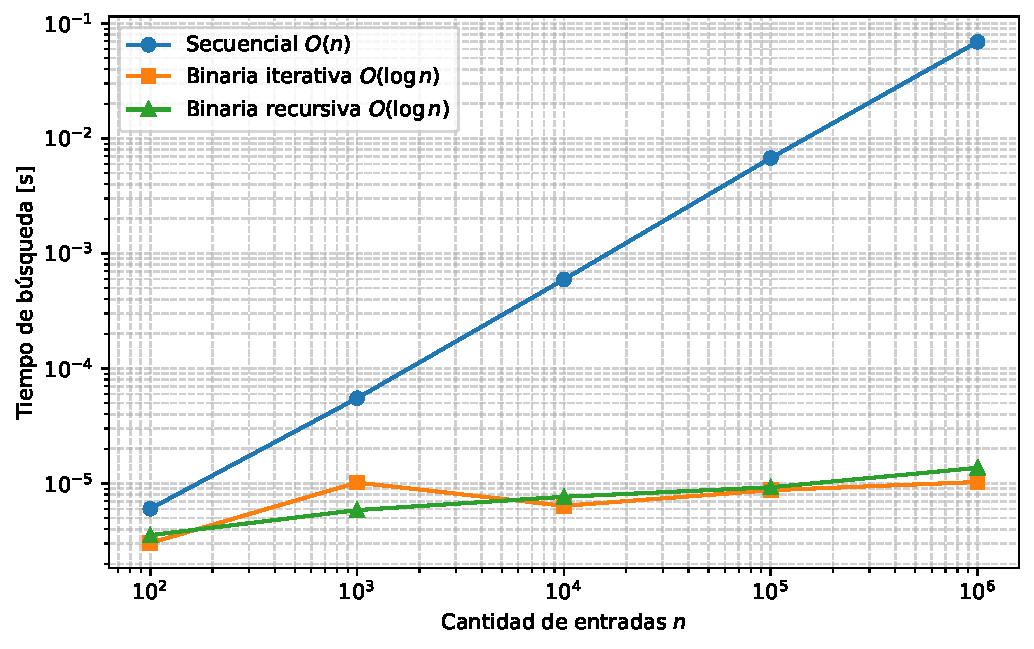
\includegraphics[width=0.75\linewidth]{figuras/benchmark_busqueda.pdf}
\caption{Comparación empírica del costo de búsqueda secuencial y binaria en el
registro de paquetes (escala log-log).}
\label{fig:bench}
\end{figure}

Los tiempos coinciden con el análisis. Cada vez que $n$ se multiplica por 10,
el tiempo de la búsqueda secuencial también se multiplica por cerca de 10, que
es el comportamiento lineal esperado. La búsqueda binaria pasa de unos 3 a unos
10~$\mu$s mientras $n$ crece cuatro órdenes de magnitud, como corresponde a un
crecimiento logarítmico. Para $n = 10^6$ la búsqueda binaria es unas 6700 veces
más rápida que la secuencial. La versión recursiva es algo más lenta que la
iterativa en los tamaños grandes por el costo de las llamadas. El valor de la
binaria iterativa en $n = 10^3$ se aparta de la tendencia; con tiempos de pocos
microsegundos y solo cinco repeticiones, la medición es sensible al ruido del
sistema.

\subsection{Pruebas}

El archivo \texttt{tests/test\_enlace.py} contiene siete pruebas automáticas
(\texttt{python -m pytest}): recepción de un paquete correcto con la potencia
esperada, los cuatro casos de error (sin ruta, TTL expirado, MAC incorrecta y
potencia bajo el umbral), el orden y la capacidad de la cola FIFO, y la
equivalencia de las tres búsquedas. Las siete pasan.

\section{Flujo de trabajo en Git}

El desarrollo se hizo con una rama por funcionalidad, integrada a \texttt{main}
mediante \textit{pull requests}. La Tabla~\ref{tab:git} lista los integrados
hasta la fecha, todos el 10 de noviembre de 2026.

\begin{table}[h]
\centering
\caption{\textit{Pull requests} integrados a \texttt{main}.}
\label{tab:git}
\begin{tabular}{cl}
\toprule
PR & Rama \\
\midrule
\#1 & \texttt{feature/hito2-refactor} \\
\#2 & \texttt{volver-version-original} \\
\#3 & \texttt{separar-modulos} \\
\#4 & \texttt{arreglar-componente} \\
\#5 & \texttt{busqueda-binaria} \\
\#6, \#7 & \texttt{hito2\_Alejandro\_hashing} \\
\bottomrule
\end{tabular}
\end{table}

El PR \#1 se revirtió con el PR \#2 para volver a la versión original, y
después el código se separó en módulos con el PR \#3. El encapsulamiento de los
canales y el módulo de simulación se desarrollaron en la rama
\texttt{fix/encapsulamiento-y-rutas}, y sobre ella la rama
\texttt{hito2-correcciones} agrega la cola FIFO, la transmisión real de los
paquetes y las pruebas.

\section{Conclusiones}

El simulador transmite los paquetes de extremo a extremo y registra el
resultado real de cada uno. Las tres estructuras elegidas responden a una
necesidad concreta del problema: la tabla hash resuelve el siguiente salto en
$O(1)$, la cola FIFO despacha los paquetes en $O(1)$ y conserva el orden que
la búsqueda binaria necesita, y la búsqueda binaria permite auditar un paquete
en $O(\log n)$ en lugar de $O(n)$. Las mediciones confirman el análisis: con un
millón de entradas, la búsqueda binaria es más de tres órdenes de magnitud más
rápida que la secuencial.

Como trabajo para la entrega final queda construir las tablas de rutas de
forma automática en vez de cargarlas a mano, y evaluar topologías con más de
un camino entre transmisor y receptor.

\end{document}
